\chapter{Suppl\texorpdfstring{ementary}{.} material for Chap\texorpdfstring{ter}{.}
\getrefnumber{ch:Integration}}\label{ch:SupplIntegration}
%\chaptermark{Supplementary material for \getrefnumber{ch:Integration}}


\section{Hypergeometric test}\label{sec:hypergeometricTest}

The hypergeometric test uses the hypergeometric distribution
and equates to the one-sided Fisher's exact test.
It allows measuring the statistical significance of
randomly sampling $k$ successes out of $n$ draws, without replacement,
from a population of $N$ that contains $K$ successes.
Depending on whether the test is about an over or under-representation,
the p-value is the probability of drawing respectively
a minimum or a maximum of $k$ successes.\mybr\

See also \citet{Johnson2005-mf} for more examples using this test.\mybr\


\begin{figure}[!htb]
    \includegraphics[scale=0.61]{integration/Kidney_scattplot_Q1_T15pv.png}\centering
    \caption[Scatterplot of protein (Pandey \etal\ --- Top3 quantification)
    and \mRNA\ (Uhlén \etal) expression for Kidney]{\label{fig:ScatKidQ1}%
    \textbf{Scatterplot of protein (Pandey \etal\ --- Top3 quantification)
    and \mRNA\ (Uhlén \etal) expression for Kidney.}}
\end{figure}


\begin{figure}[htp]
    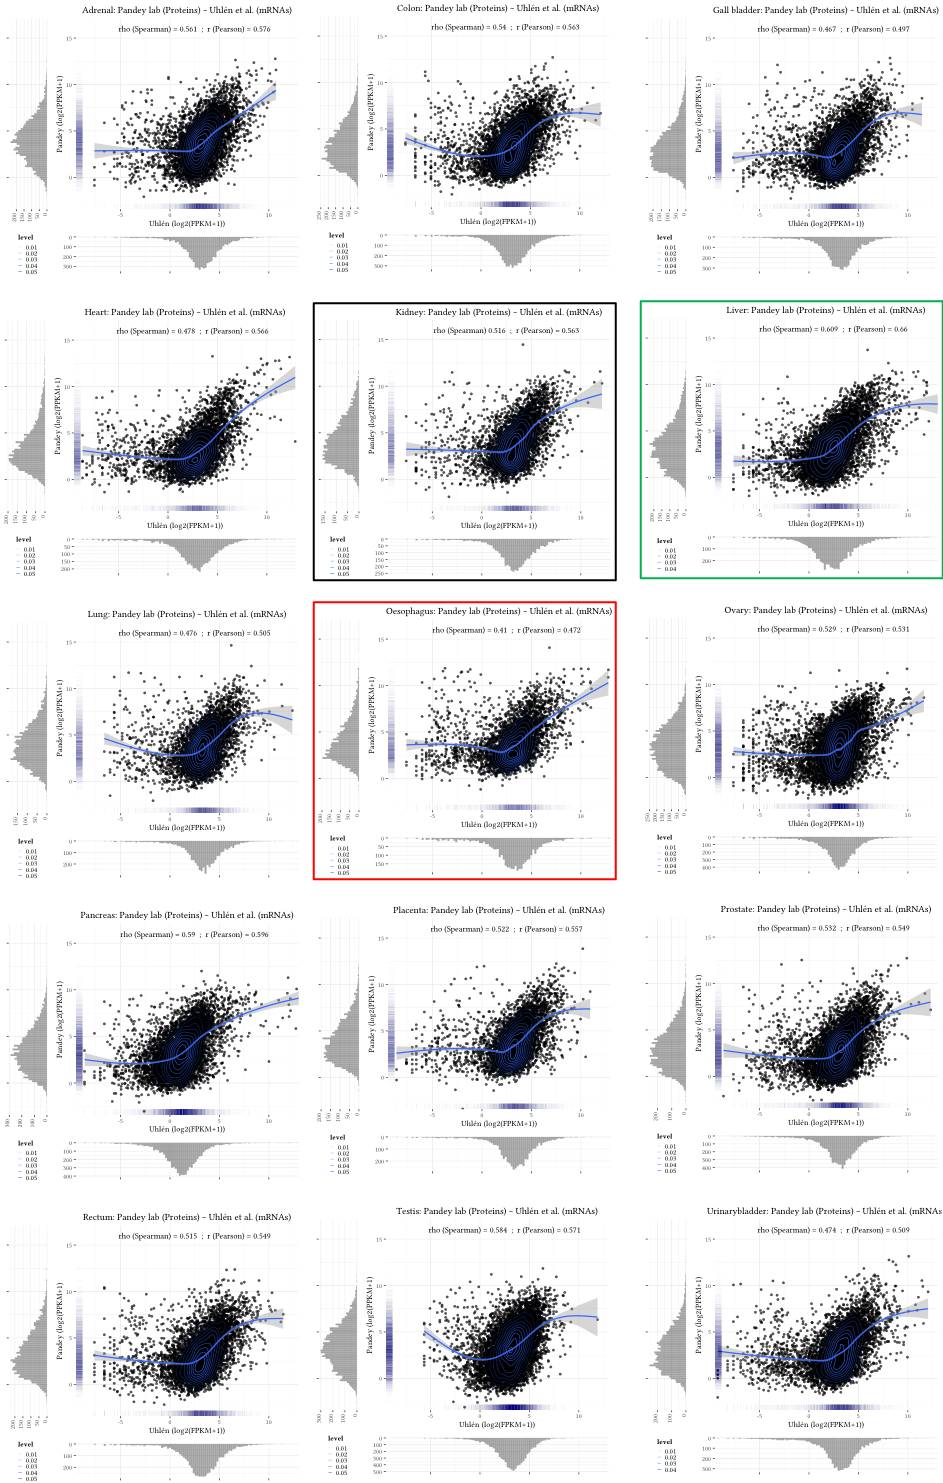
\includegraphics[scale=0.85]{integration/scatplotsQ3T15.png}\centering
    \caption[Overview of the tissue scatterplots between Uhlén and Pandey data]{%
    \label{fig:scatplotAll}\textbf{Overview of the tissue scatterplots
    between Uhlén and Pandey data.}
    The \liver\ presents the highest correlation and the \oesophagus\ the lowest one.}
\end{figure}

\pagestyle{plain}
\small

\begin{landscape}
    \begin{longtable}{@{}llllll@{}}%[]%\centering
    \caption{Found proteins without a counterpart in the transcriptomic data}\label{tab:protNoTrans}\\
\toprule
Set & ENSEMBL (76) ID & Gene name & Biotype & Description & \begin{tabular}[c]{@{}l@{}}Source and \\ Accessing number\end{tabular} \\* \midrule
\endfirsthead
    \caption[]{Found proteins without a counterpart in the transcriptomic data}\\
\toprule
Set & ENSEMBL (76) ID & Gene name & Biotype & Description & \begin{tabular}[c]{@{}l@{}}Source and \\ Accessing number\end{tabular} \\* \midrule
\endhead
%
\bottomrule
\endfoot
%
\endlastfoot
%
a, b, c, d & ENSG00000173349 & SFT2D3 & p.\ coding & SFT2 domain containing 3 & \begin{tabular}[c]{@{}l@{}}HGNC Symbol \\ Acc: 28767\end{tabular} \\
a, b & ENSG00000198788 & MUC2 & \begin{tabular}[c]{@{}l@{}}processed\\ transcript\end{tabular} & \begin{tabular}[c]{@{}l@{}}mucin 2, \\ oligomeric mucus/gel-forming\end{tabular} & \begin{tabular}[c]{@{}l@{}}HGNC Symbol\\ Acc: 7512\end{tabular} \\
a, b, c, d & ENSG00000223953 & C1QTNF5 & p.\ coding & \begin{tabular}[c]{@{}l@{}}C1q and tumor necrosis\\ factor related protein 5\end{tabular} & \begin{tabular}[c]{@{}l@{}}HGNC Symbol\\ Acc:14344\end{tabular} \\
a, b & ENSG00000256453 & DND1 & p.\ coding & \begin{tabular}[c]{@{}l@{}}DND microRNA-mediated \\ repression inhibitor\end{tabular} & \begin{tabular}[c]{@{}l@{}}HGNC Symbol\\ Acc:23799\end{tabular} \\
a, b, c, d & ENSG00000262664 & OVCA2 & p.\ coding & \begin{tabular}[c]{@{}l@{}}ovarian tumor suppressor\\ candidate 2\end{tabular} & \begin{tabular}[c]{@{}l@{}}HGNC Symbol\\ Acc:24203\end{tabular} \\
b & ENSG00000163157 & TMOD4 & p.\ coding & tropomodulin 4 (muscle) & \begin{tabular}[c]{@{}l@{}}HGNC Symbol\\ Acc:11874\end{tabular} \\
b & ENSG00000203618 & GP1BB & p.\ coding & \begin{tabular}[c]{@{}l@{}}glycoprotein Ib (platelet), \\ beta polypeptide\end{tabular} & \begin{tabular}[c]{@{}l@{}}HGNC Symbol\\ Acc:4440\end{tabular} \\
b & ENSG00000251322 & SHANK3 & \begin{tabular}[c]{@{}l@{}}processed\\ transcript\end{tabular} & \begin{tabular}[c]{@{}l@{}}SH3 and \\ multiple ankyrin repeat domains 3\end{tabular} & \begin{tabular}[c]{@{}l@{}}HGNC Symbol\\ Acc:14294\end{tabular} \\
c, d & ENSG00000105371 & ICAM4 & p.\ coding & \begin{tabular}[c]{@{}l@{}}intercellular adhesion molecule 4 \\ (Landsteiner-Wiener blood group)\end{tabular} & \begin{tabular}[c]{@{}l@{}}HGNC Symbol\\ Acc:5347\end{tabular} \\
c & ENSG00000164708 & PGAM2 & p.\ coding & phosphoglycerate mutase 2 (muscle) & \begin{tabular}[c]{@{}l@{}}HGNC Symbol \\ Acc:8889\end{tabular} \\
c, d & ENSG00000181404 & XXyac-YRM2039.2 & \begin{tabular}[c]{@{}l@{}}unprocesssed\\ pseudogene\end{tabular} &  &  \\
c, d & ENSG00000183336 & BOLA2 & p.\ coding & bolA family member 2 & \begin{tabular}[c]{@{}l@{}}HGNC Symbol\\ Acc:29488\end{tabular} \\
c & ENSG00000196101 & HLA-DRB3 & p.\ coding & \begin{tabular}[c]{@{}l@{}}major histocompatibility complex, \\ class II, DR beta 3\end{tabular} & \begin{tabular}[c]{@{}l@{}}HGNC Symbol\\ Acc:4951\end{tabular} \\
c & ENSG00000203618 & GP1BB &  & \begin{tabular}[c]{@{}l@{}}glycoprotein Ib (platelet), \\ beta polypeptide\end{tabular} & \begin{tabular}[c]{@{}l@{}}HGNC Symbol\\ Acc:4440\end{tabular} \\
c, d & ENSG00000206203 & TSSK2 & p.\ coding & testis-specific serine kinase 2 & \begin{tabular}[c]{@{}l@{}}HGNC Symbol\\ Acc:1140\end{tabular} \\
c, d & \begin{tabular}[c]{@{}c@{}}ENSG00000206240,\\ ENSG00000206306\end{tabular} & HLA-DRB1 & p.\ coding & \begin{tabular}[c]{@{}l@{}}major histocompatibility complex, \\ class II, DR beta 1\end{tabular} & \begin{tabular}[c]{@{}l@{}}HGNC Symbol\\ Acc:4948\end{tabular} \\
c, d & ENSG00000206305 & HLA-DQA1 &  & \begin{tabular}[c]{@{}l@{}}major histocompatibility complex,\\ class II, DQ alpha 1\end{tabular} & \begin{tabular}[c]{@{}l@{}}HGNC Symbol\\ Acc:4942\end{tabular} \\
c, d & \begin{tabular}[c]{@{}c@{}}ENSG00000206450,\\ ENSG00000223532\end{tabular} & HLA-B & p.\ coding & \begin{tabular}[c]{@{}l@{}}major histocompatibility complex, \\ class I, B\end{tabular} & \begin{tabular}[c]{@{}l@{}}HGNC Symbol \\ Acc:4932\end{tabular} \\
c, d & ENSG00000225691 & HLA-C & p.\ coding & \begin{tabular}[c]{@{}l@{}}major histocompatibility complex, \\ class I, C\end{tabular} & \begin{tabular}[c]{@{}l@{}}HGNC Symbol\\ Acc:4933\end{tabular} \\
c, d & \begin{tabular}[c]{@{}c@{}}ENSG00000206505,\\ ENSG00000224320,\\ ENSG00000227715,\\ ENSG00000235657,\\ ENSG00000223980,\\ ENSG00000229215\end{tabular} & HLA-A & p.\ coding & \begin{tabular}[c]{@{}l@{}}major histocompatibility complex,\\ class I, A\end{tabular} & \begin{tabular}[c]{@{}l@{}}HGNC Symbol\\ Acc:4931\end{tabular} \\
c, d & ENSG00000211594 & IGKJ4 & IG J gene & immunoglobulin kappa joining 4 & \begin{tabular}[c]{@{}l@{}}HGNC Symbol\\ Acc:5722\end{tabular} \\
c, d & ENSG00000211595 & IGKJ3 & IG J gene & immunoglobulin kappa joining 3 & \begin{tabular}[c]{@{}l@{}}HGNC Symbol\\ Acc:5721\end{tabular} \\
c & ENSG00000213402 & PTPRCAP & p.\ coding & \begin{tabular}[c]{@{}l@{}}protein tyrosine phosphatase,\\ receptor type, C-associated protein\end{tabular} & \begin{tabular}[c]{@{}l@{}}HGNC Symbol\\ Acc:9667\end{tabular} \\
c & ENSG00000215695 & RSC1A1 & p.\ coding & \begin{tabular}[c]{@{}l@{}}regulatory solute carrier protein, \\ family 1, member 1\end{tabular} & \begin{tabular}[c]{@{}l@{}}HGNC Symbol\\ Acc:10458\end{tabular} \\
c, d & ENSG00000227357 & HLA-DRB4 & p.\ coding & \begin{tabular}[c]{@{}l@{}}major histocompatibility complex, \\ class II, DR beta 4\end{tabular} & \begin{tabular}[c]{@{}l@{}}HGNC Symbol\\ Acc:4952\end{tabular} \\
c, d & ENSG00000231021 & HLA-DRB4 & p.\ coding & \begin{tabular}[c]{@{}l@{}}major histocompatibility complex,\\ class II, DR beta 4\end{tabular} & \begin{tabular}[c]{@{}l@{}}RefSeq mRNA\\ Acc:NM\_021983\end{tabular} \\
c, d & ENSG00000231286 & HLA-DQB1 & p.\ coding & \begin{tabular}[c]{@{}l@{}}major histocompatibility complex, \\ class II, DQ beta 1\end{tabular} & \begin{tabular}[c]{@{}l@{}}HGNC Symbol\\ Acc:4944\end{tabular} \\
c, d & ENSG00000231679 & HLA-DRB3 & p.\ coding & \begin{tabular}[c]{@{}l@{}}major histocompatibility complex,\\ class II, DR beta 3\end{tabular} & \begin{tabular}[c]{@{}l@{}}RefSeq mRNA\\ Acc:NM\_022555\end{tabular} \\
c, d & ENSG00000256453 & DND1 & p.\ coding & \begin{tabular}[c]{@{}l@{}}DND microRNA-mediated \\ repression inhibitor\end{tabular} & \begin{tabular}[c]{@{}l@{}}HGNC Symbol\\ Acc:23799\end{tabular} \\
c & ENSG00000263353 & CH17-118O6.1 & \begin{tabular}[c]{@{}l@{}}processed \\ transcript\end{tabular} &  &  \\
c, d & ENSG00000276938 & FAM157A & p.\ coding & \begin{tabular}[c]{@{}l@{}}Homo sapiens family with \\ sequence similarity 157, member A\end{tabular} & \begin{tabular}[c]{@{}l@{}}RefSeq mRNA\\ Acc:NM\_001145248\end{tabular} \\
c, d & ENSG00000277656 & GSTT1 & p.\ coding & glutathione S-transferase theta 1 & \begin{tabular}[c]{@{}l@{}}HGNC Symbol\\ Acc:4641\end{tabular} \\
c, d & ENSG00000277897 & GSTT2 & p.\ coding &  &  \\
d & ENSG00000105507 & CABP5 & p.\ coding & calcium binding protein 5 & \begin{tabular}[c]{@{}l@{}}HGNC Symbol\\ Acc:3714\end{tabular} \\
d & ENSG00000105954 & NPVF & p.\ coding & neuropeptide VF precursor & \begin{tabular}[c]{@{}l@{}}HGNC Symbol\\ Acc:13782\end{tabular} \\
d & ENSG00000142539 & CTD-2545M3.6 & p.\ coding &  &  \\
d & ENSG00000147896 & IFNK & p.\ coding & interferon, kappa & \begin{tabular}[c]{@{}l@{}}HGNC Symbol\\ Acc:21714\end{tabular} \\
d & ENSG00000148136 & OR13C4 & p.\ coding & \begin{tabular}[c]{@{}l@{}}olfactory receptor, family 13, \\ subfamily C, member 4\end{tabular} & \begin{tabular}[c]{@{}l@{}}HGNC Symbol\\ Acc:4722\end{tabular} \\
d & ENSG00000163157 & TMOD & p.\ coding & tropomodulin 4 (muscle) & \begin{tabular}[c]{@{}l@{}}HGNC Symbol\\ Acc:11874\end{tabular} \\
d & ENSG00000164708 & PGAM2 & p.\ coding & \begin{tabular}[c]{@{}l@{}}phosphoglycerate mutase 2\\ (muscle)\end{tabular} & \begin{tabular}[c]{@{}l@{}}HGNC Symbol\\ Acc:8889\end{tabular} \\
d & ENSG00000166884 & OR4D6 & p.\ coding & \begin{tabular}[c]{@{}l@{}}olfactory receptor, family 4, \\ subfamily D, member 6\end{tabular} & \begin{tabular}[c]{@{}l@{}}HGNC Symbol\\ Acc:15175\end{tabular} \\
d & ENSG00000169840 & GSX1 & p.\ coding & GS homeobox 1 & \begin{tabular}[c]{@{}l@{}}HGNC Symbol\\ Acc:20374\end{tabular} \\
d & ENSG00000170929 & OR1M1 & p.\ coding & \begin{tabular}[c]{@{}l@{}}olfactory receptor, family 1, \\ subfamily M, member 1\end{tabular} & \begin{tabular}[c]{@{}l@{}}HGNC Symbol\\ Acc:8220\end{tabular} \\
d & ENSG00000171053 & PATE1 & p.\ coding & prostate and testis expressed 1 & \begin{tabular}[c]{@{}l@{}}HGNC Symbol\\ Acc:24664\end{tabular} \\
d & ENSG00000171396 & KRTAP4-4 & p.\ coding & keratin associated protein 4-4 & \begin{tabular}[c]{@{}l@{}}HGNC Symbol\\ Acc:16928\end{tabular} \\
d & ENSG00000172155 & LCE1D & p.\ coding & late cornified envelope 1D & \begin{tabular}[c]{@{}l@{}}HGNC Symbol\\ Acc:29465\end{tabular} \\
d & ENSG00000176239 & OR51B6 & p.\ coding & \begin{tabular}[c]{@{}l@{}}olfactory receptor, family 51, \\ subfamily B, member 6\end{tabular} & \begin{tabular}[c]{@{}l@{}}HGNC Symbol\\ Acc:19600\end{tabular} \\
d & ENSG00000182346 & DAOA & p.\ coding & D-amino acid oxidase activator & \begin{tabular}[c]{@{}l@{}}HGNC Symbol\\ Acc:21191\end{tabular} \\
d & ENSG00000182591 & KRTAP11-1 & p.\ coding & keratin associated protein 11-1 & \begin{tabular}[c]{@{}l@{}}HGNC Symbol\\ Acc:18922\end{tabular} \\
d & ENSG00000184321 & OR51J1 & p.\ coding & \begin{tabular}[c]{@{}l@{}}olfactory receptor, family 51, \\ subfamily J, member 1\\ (gene/pseudogene)\end{tabular} & \begin{tabular}[c]{@{}l@{}}HGNC Symbol\\ Acc:14856\end{tabular} \\
d & ENSG00000187173 & LCE2A & p.\ coding & late cornified envelope 2A & \begin{tabular}[c]{@{}l@{}}HGNC Symbol\\ Acc:29469\end{tabular} \\
d & ENSG00000187766 & KRTAP10-8 & p.\ coding & keratin associated protein 10-8 & \begin{tabular}[c]{@{}l@{}}HGNC Symbol\\ Acc:20525\end{tabular} \\
d & ENSG00000196101 & HLA-DRB3 & p.\ coding & \begin{tabular}[c]{@{}l@{}}major histocompatibility complex, \\ class II, DR beta 3\end{tabular} & \begin{tabular}[c]{@{}l@{}}HGNC Symbol\\ Acc:4951\end{tabular} \\
d & ENSG00000203618 & GP1BB & p.\ coding & \begin{tabular}[c]{@{}l@{}}glycoprotein Ib (platelet), \\ beta polypeptide\end{tabular} & \begin{tabular}[c]{@{}l@{}}HGNC Symbol\\ Acc:4440\end{tabular} \\
d & ENSG00000203818 & HIST2H3PS2 & p.\ coding & \begin{tabular}[c]{@{}l@{}}histone cluster 2, H3,\\ pseudogene 2\end{tabular} & \begin{tabular}[c]{@{}l@{}}HGNC Symbol\\ Acc:32060\end{tabular} \\
d & ENSG00000205883 & DEFB135 & p.\ coding & defensin, beta 135 & \begin{tabular}[c]{@{}l@{}}HGNC Symbol\\ Acc:32400\end{tabular} \\
d & ENSG00000206452 & HLA-C & p.\ coding & \begin{tabular}[c]{@{}l@{}}major histocompatibility complex, \\ class I, C\end{tabular} & \begin{tabular}[c]{@{}l@{}}HGNC Symbol\\ Acc:4933\end{tabular} \\
d & ENSG00000211831 & TRAJ61 & TR J gene & \begin{tabular}[c]{@{}l@{}}T cell receptor alpha joining 61\\ (non-functional)\end{tabular} & \begin{tabular}[c]{@{}l@{}}HGNC Symbol\\ Acc:12094\end{tabular} \\
d & ENSG00000211835 & TRAJ56 & TR J gene & T cell receptor alpha joining 56 & \begin{tabular}[c]{@{}l@{}}HGNC Symbol\\ Acc:12088\end{tabular} \\
d & ENSG00000213316 & LTC4S & p.\ coding & leukotriene C4 synthase & \begin{tabular}[c]{@{}l@{}}HGNC Symbol\\ Acc:6719\end{tabular} \\
d & ENSG00000213402 & PTPRCAP & p.\ coding & \begin{tabular}[c]{@{}l@{}}protein tyrosine phosphatase, \\ receptor type, C-associated protein\end{tabular} & \begin{tabular}[c]{@{}l@{}}HGNC Symbol\\ Acc:9667\end{tabular} \\
d & ENSG00000215695 & RSC1A1 & p.\ coding & \begin{tabular}[c]{@{}l@{}}regulatory solute carrier protein, \\ family 1, member 1\end{tabular} & \begin{tabular}[c]{@{}l@{}}HGNC Symbol\\ Acc:10458\end{tabular} \\
d & ENSG00000224902 & GAGE12H & p.\ coding & G antigen 12H & \begin{tabular}[c]{@{}l@{}}HGNC Symbol\\ Acc:31908\end{tabular} \\
d & ENSG00000233732 & IGHV3OR16-10 & IG V gene & \begin{tabular}[c]{@{}l@{}}immunoglobulin heavy variable 3\\ OR16-10 (non-functional)\end{tabular} & \begin{tabular}[c]{@{}l@{}}HGNC Symbol\\ Acc:5634\end{tabular} \\
d & ENSG00000249209 & AP000304.12 & p.\ coding &  &  \\
d & ENSG00000249730 & OR10J4 & \begin{tabular}[c]{@{}l@{}}polymorphic\\ pseudogene\end{tabular} & \begin{tabular}[c]{@{}l@{}}olfactory receptor, \\ family 10, subfamily J,\\ member 4 (gene/pseudogene)\end{tabular} & \begin{tabular}[c]{@{}l@{}}HGNC Symbol\\ Acc:15408\end{tabular} \\
d & ENSG00000253148 & RGS21 & p.\ coding & regulator of G-protein signaling 21 & \begin{tabular}[c]{@{}l@{}}HGNC Symbol\\ Acc:26839\end{tabular} \\
d & ENSG00000255009 & UBTFL1 & \begin{tabular}[c]{@{}l@{}}processed \\ pseudogene\end{tabular} & \begin{tabular}[c]{@{}l@{}}upstream binding transcription factor,\\ RNA polymerase I-like 1\end{tabular} & \begin{tabular}[c]{@{}l@{}}HGNC Symbol\\ Acc:14533\end{tabular} \\
d & ENSG00000255472 & RP11-998D10.1 & p.\ coding & uncharacterized protein & \begin{tabular}[c]{@{}l@{}}UniProtKB/TrEMBL\\ Acc:E9PR74\end{tabular} \\
d & ENSG00000259490 & IGHV3OR15-7 & IG V gene & \begin{tabular}[c]{@{}l@{}}immunoglobulin heavy variable 3\\ OR15-7 (pseudogene)\end{tabular} & \begin{tabular}[c]{@{}l@{}}HGNC Symbol\\ Acc:5633\end{tabular} \\
d & ENSG00000263353 & CH17-118O6.1 & \begin{tabular}[c]{@{}l@{}}processed\\ transcript\end{tabular} &  &  \\
d & ENSG00000270467 & IGHV3OR16-12 & IG V gene & \begin{tabular}[c]{@{}l@{}}immunoglobulin heavy variable 3\\ OR16-12 (non-functional)\end{tabular} & \begin{tabular}[c]{@{}l@{}}HGNC Symbol\\ Acc:5636\end{tabular} \\
d & ENSG00000270472 & IGHV3OR16-9 & IG V gene & \begin{tabular}[c]{@{}l@{}}immunoglobulin heavy variable 3\\ OR16-9 (non-functional)\end{tabular} & \begin{tabular}[c]{@{}l@{}}HGNC Symbol\\ Acc:5644\end{tabular} \\*
    \bottomrule
\end{longtable}

\begin{figure}[bp]
    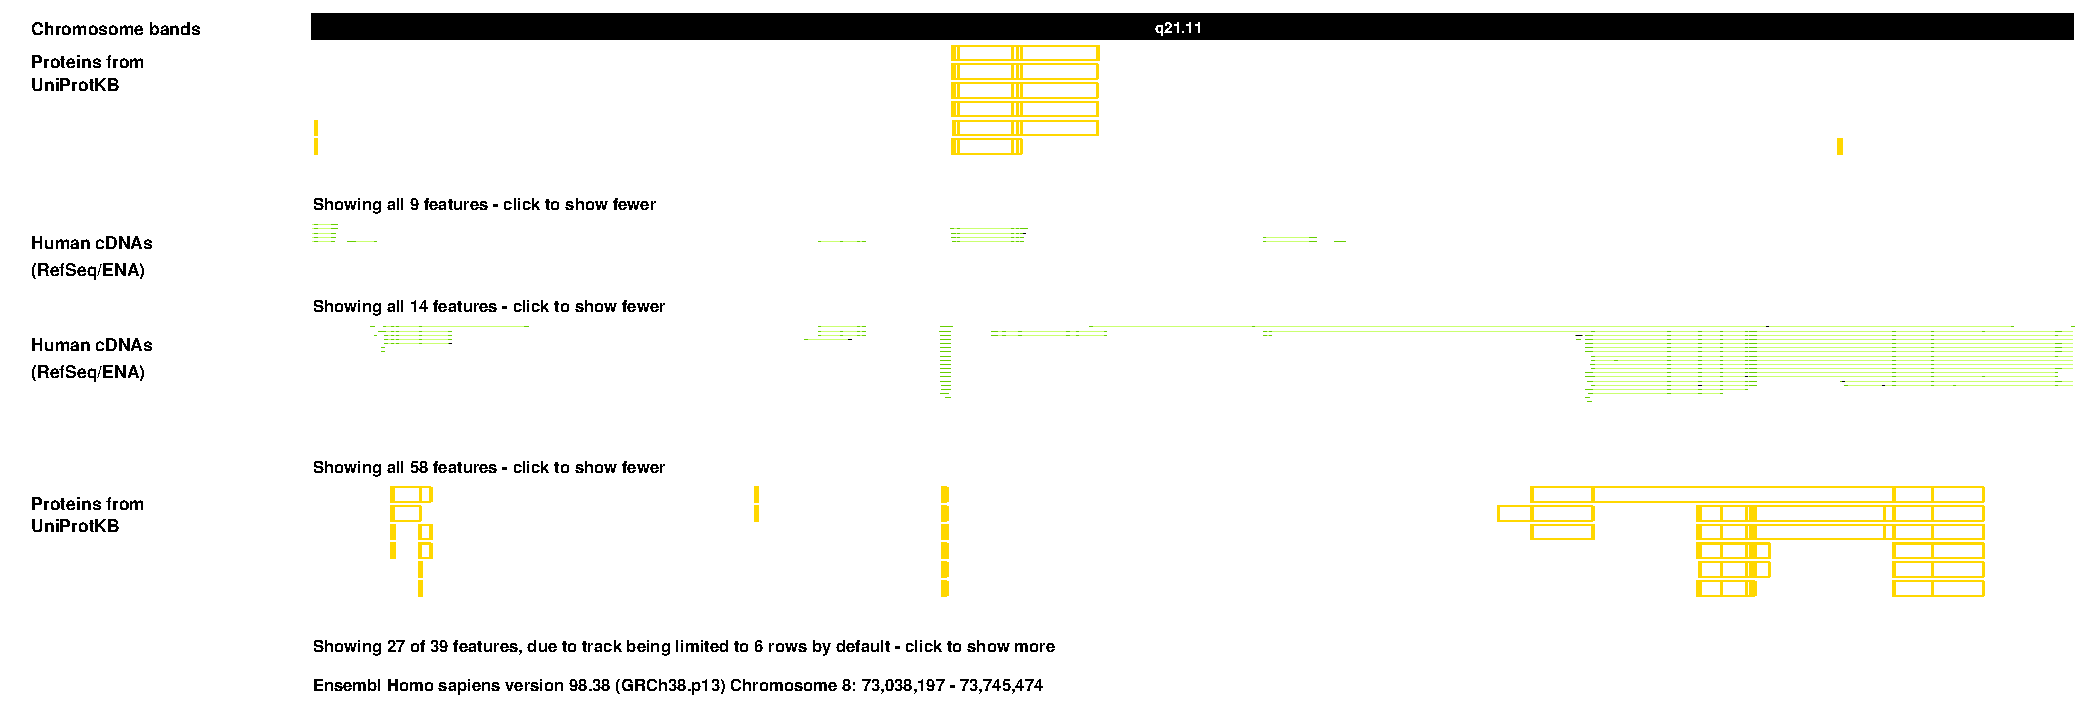
\includegraphics[scale=0.5]{integration/Human_873038197_73745474}\centering
    \caption[STAU2 definition]{\label{fig:stau2def}\textbf{\gene{STAU2} definition}
    The chromosome annotations for the \mRNA\ and the protein of \gene{STAU2}
    are different.}
\end{figure}

\end{landscape}

\pagestyle{scrheadings}
\normalsize

\begin{figure}[!htpb]
    \includegraphics[scale=0.8]{integration/DFtest2.pdf}\centering
    \vspace{-3.5mm}
    \caption[Distribution of Pearson and Spearman correlation coefficients
    for same-tissue proteomic and transcriptomic pairs
    versus random tissue pairs (untransformed data)]{\label{fig:TestSigUnlog}%
    \textbf{Distribution of Pearson and Spearman correlation coefficients
    for same-tissue proteomic and transcriptomic pairs versus random tissue
    pairs (untransformed data).}}
\end{figure}

\pagestyle{plain}
\begin{landscape}
\begin{longtable}{@{}ccccccccc@{}}
\caption[Summary of Pearson and Spearman correlations
between proteomics and transcriptomics]{\label{tab:pvalueCorrSP}%
\textbf{Summary of Pearson and Spearman correlation coefficients
between proteomics and transcriptomics} across several data combinations.
See also \Cref{fig:TestSig}.}\\
\toprule
\multicolumn{2}{c}{} &  &  &  &  & \multicolumn{2}{c}{Mean correlation of} &  \\* \cmidrule(lr){7-8}
\multicolumn{2}{c}{\multirow{-2}{*}{Datasets}} & \multirow{-2}{*}{\begin{tabular}[c]{@{}c@{}}Number \\ of tissues\end{tabular}} & \multirow{-2}{*}{\begin{tabular}[c]{@{}c@{}}Quantification\\ methods\end{tabular}} & \multirow{-2}{*}{\begin{tabular}[c]{@{}c@{}}Scaled data\\ $\log_2(x+1)$\end{tabular}} & \multirow{-2}{*}{\begin{tabular}[c]{@{}c@{}}Correlation\\ method\end{tabular}} & Same-tissue pairs & Different tissues pairs & \multirow{-2}{*}{p-value} \\* \midrule
\endfirsthead
\caption[]{\textbf{Summary of Pearson and Spearman correlation coefficients
between proteomics and transcriptomics} across several data combinations.
See also \Cref{fig:TestSig}.}\\
\toprule
\multicolumn{2}{c}{} &  &  &  &  & \multicolumn{2}{c}{Mean correlation of} &  \\* \cmidrule(lr){7-8}
\multicolumn{2}{c}{\multirow{-2}{*}{Datasets}} & \multirow{-2}{*}{\begin{tabular}[c]{@{}c@{}}Number \\ of tissues\end{tabular}} & \multirow{-2}{*}{\begin{tabular}[c]{@{}c@{}}Quantification\\ methods\end{tabular}} & \multirow{-2}{*}{\begin{tabular}[c]{@{}c@{}}Scaled data\\ $\log_2(x+1)$\end{tabular}} & \multirow{-2}{*}{\begin{tabular}[c]{@{}c@{}}Correlation\\ method\end{tabular}} & Same-tissue pairs & Different tissues pairs & \multirow{-2}{*}{p-value} \\* \midrule
\endhead
%
\bottomrule
\endfoot
%
\endlastfoot
%
Pandey \etal\ & Uhlén \etal\ & 12 & Top3 x HTSeq & True & Spearman & 0.51 & 0.37 & 4.66e-07 \\
Pandey \etal\ & GTEx & 12 & Top3 x HTSeq & True & Spearman & 0.5 & 0.37 & 7.379e-07 \\
{\color[HTML]{9B9B9B} Uhlén \etal} & {\color[HTML]{9B9B9B} GTEx} & {\color[HTML]{9B9B9B} 12} & {\color[HTML]{9B9B9B} HTSeq x HTSeq} & {\color[HTML]{9B9B9B} True} & {\color[HTML]{9B9B9B} Spearman} & {\color[HTML]{9B9B9B} 0.91} & {\color[HTML]{9B9B9B} 0.66} & {\color[HTML]{9B9B9B} \textless\ 2.2e-16} \\
Pandey \etal\ & Uhlén \etal\ & 15 & Top3 x HTSeq & True & Spearman & 0.5 & 0.38 & 2.659e-08 \\
Pandey \etal\ & Uhlén \etal\ & 12 & Top3 x HTSeq & True & Pearson & 0.11 & 0.06 & 0.03696 \\
Pandey \etal\ & GTEx & 12 & Top3 x HTSeq & True & Pearson & 0.12 & 0.07 & 0.02895 \\
{\color[HTML]{9B9B9B} Uhlén \etal} & {\color[HTML]{9B9B9B} GTEx} & {\color[HTML]{9B9B9B} 12} & {\color[HTML]{9B9B9B} HTSeq x HTSeq} & {\color[HTML]{9B9B9B} True} & {\color[HTML]{9B9B9B} Pearson} & {\color[HTML]{9B9B9B} 0.93} & {\color[HTML]{9B9B9B} 0.68} & {\color[HTML]{9B9B9B} \textless\ 2.2e-16} \\
Pandey \etal\ & Uhlén \etal\ & 15 & Top3 x HTSeq & True & Pearson & 0.1 & 0.06 & 0.02271 \\
Pandey \etal\ & Uhlén \etal\ & 12 & PPKM x HTSeq & True & Spearman & 0.52 & 0.42 & 4.795e-05 \\
Pandey \etal\ & GTEx & 12 & PPKM x HTSeq & True & Spearman & 0.52 & 0.43 & 8.475e-05 \\
{\color[HTML]{9B9B9B} Uhlén \etal} & {\color[HTML]{9B9B9B} GTEx} & {\color[HTML]{9B9B9B} 12} & {\color[HTML]{9B9B9B} HTSeq x HTSeq} & {\color[HTML]{9B9B9B} True} & {\color[HTML]{9B9B9B} Spearman} & {\color[HTML]{9B9B9B} 0.92} & {\color[HTML]{9B9B9B} 0.72} & {\color[HTML]{9B9B9B} \textless\ 2.2e-16} \\
Pandey \etal\ & Uhlén \etal\ & 15 & PPKM x HTSeq & True & Spearman & 0.52 & 0.43 & 8.422e-06 \\
Pandey \etal\ & Uhlén \etal\ & 12 & PPKM x HTSeq & True & Pearson & 0.5 & 0.37 & 0.0004002 \\
Pandey \etal\ & GTEx & 12 & PPKM x HTSeq & True & Pearson & 0.5 & 0.41 & 0.0003306 \\
{\color[HTML]{9B9B9B} Uhlén \etal} & {\color[HTML]{9B9B9B} GTEx} & {\color[HTML]{9B9B9B} 12} & {\color[HTML]{9B9B9B} HTSeq x HTSeq} & {\color[HTML]{9B9B9B} True} & {\color[HTML]{9B9B9B} Pearson} & {\color[HTML]{9B9B9B} 0.94} & {\color[HTML]{9B9B9B} 0.73} & {\color[HTML]{9B9B9B} \textless\ 2.2e-16} \\
Pandey \etal\ & Uhlén \etal\ & 15 & PPKM x HTSeq & True & Pearson & 0.49 & 0.4 & 9.941e-05 \\* \midrule
Pandey \etal\ & Uhlén \etal\ & 12 & Top3 x HTSeq & False & Spearman & 0.51 & 0.37 & 4.66e-07 \\
Pandey \etal\ & GTEx & 12 & Top3 x HTSeq & False & Spearman & 0.5 & 0.37 & 7.379e-07 \\
{\color[HTML]{9B9B9B} Uhlén \etal} & {\color[HTML]{9B9B9B} GTEx} & {\color[HTML]{9B9B9B} 12} & {\color[HTML]{9B9B9B} HTSeq x HTSeq} & {\color[HTML]{9B9B9B} False} & {\color[HTML]{9B9B9B} Spearman} & {\color[HTML]{9B9B9B} 0.91} & {\color[HTML]{9B9B9B} 0.66} & {\color[HTML]{9B9B9B} \textless\ 2.2e-16} \\
Pandey \etal\ & Uhlén \etal\ & 15 & Top3 x HTSeq & False & Spearman & 0.5 & 0.38 & 2.66e-08 \\
Pandey \etal\ & Uhlén \etal\ & 12 & Top3 x HTSeq & False & Pearson & 0.17 & 0.09 & 0.022 \\
Pandey \etal\ & GTEx & 12 & Top3 x HTSeq & False & Pearson & 0.17 & 0.1 & 0.015 \\
{\color[HTML]{9B9B9B} Uhlén \etal} & {\color[HTML]{9B9B9B} GTEx} & {\color[HTML]{9B9B9B} 12} & {\color[HTML]{9B9B9B} HTSeq x HTSeq} & {\color[HTML]{9B9B9B} False} & {\color[HTML]{9B9B9B} Pearson} & {\color[HTML]{9B9B9B} 0.92} & {\color[HTML]{9B9B9B} 0.64} & {\color[HTML]{9B9B9B} \textless\ 2.2e-16} \\
Pandey \etal\ & Uhlén \etal\ & 15 & Top3 x HTSeq & False & Pearson & 0.16 & 0.1 & 0.012 \\
Pandey \etal\ & Uhlén \etal\ & 12 & PPKM x HTSeq & False & Spearman & 0.52 & 0.42 & 4.795e-05 \\
Pandey \etal\ & GTEx & 12 & PPKM x HTSeq & False & Spearman & 0.52 & 0.43 & 8.475e-05 \\
{\color[HTML]{9B9B9B} Uhlén \etal} & {\color[HTML]{9B9B9B} GTEx} & {\color[HTML]{9B9B9B} 12} & {\color[HTML]{9B9B9B} HTSeq x HTSeq} & {\color[HTML]{9B9B9B} False} & {\color[HTML]{9B9B9B} Spearman} & {\color[HTML]{9B9B9B} 0.92} & {\color[HTML]{9B9B9B} 0.72} & {\color[HTML]{9B9B9B} \textless\ 2.2e-16} \\
Pandey \etal\ & Uhlén \etal\ & 15 & PPKM x HTSeq & False & Spearman & 0.52 & 0.43 & 8.422e-06 \\
Pandey \etal\ & Uhlén \etal\ & 12 & PPKM x HTSeq & False & Pearson & 0.55 & 0.43 & 1.059e-06 \\
Pandey \etal\ & GTEx & 12 & PPKM x HTSeq & False & Pearson & 0.56 & 0.45 & 2.026e-06 \\
{\color[HTML]{9B9B9B} Uhlén \etal} & {\color[HTML]{9B9B9B} GTEx} & {\color[HTML]{9B9B9B} 12} & {\color[HTML]{9B9B9B} HTSeq x HTSeq} & {\color[HTML]{9B9B9B} False} & {\color[HTML]{9B9B9B} Pearson} & {\color[HTML]{9B9B9B} 0.93} & {\color[HTML]{9B9B9B} 0.69} & {\color[HTML]{9B9B9B} \textless\ 2.2e-16} \\
Pandey \etal\ & Uhlén \etal\ & 15 & PPKM x HTSeq & False & Pearson & 0.55 & 0.45 & 1.061e-07 \\* \bottomrule
\end{longtable}
\end{landscape}


\pagestyle{scrheadings}

\begin{figure}[!htpb]
    \includegraphics[scale=0.6]{integration/compCorJind.pdf}\centering
    \caption[Rank comparison chart]{\label{fig:compCorJind}\textbf{Rank comparison
    between the Pearson/Spearman correlation and the Jaccard indices
    computed for matching proteomics and transcriptomics.}}
\end{figure}

\begin{comment}
\begin{figure}[!htb]
    \includegraphics[scale=0.7]{integration/TissuePairsQ3T15HeatmapPandey.pdf}\centering
    \vspace{-8mm}
    \caption[Number of shared genes between tissue couples of Pandey (PPKM quantification)]{%
    \label{fig:heatmapPandeyTissuePairs}\textbf{Number of shared genes
    between tissue couples of Pandey Lab data (PPKM quantification).} The hierarchical
    tree of the tissues is based on their relative closeness
    (tissues that share a higher number of commun genes are closer).
    The groups are linked with the Ward method.}
\end{figure}

\begin{figure}[!htb]
    \includegraphics[scale=0.7]{integration/TissuePairsQ3T15HeatmapUhlen05.pdf}\centering
    \vspace{-8mm}
    \caption[Number of shared genes between tissue couples of Pandey (12,921 genes)]{%
    \label{fig:heatmapUhlenTissuePairs05}\textbf{Number of shared genes
    between tissue couples of Uhlén et al.\ data (12,921 commun genes set
    across the fifteen shared tissues with Pandey Lab data quantified
    with PPKM method)} The
    hierarchical tree share the same parameters than \Cref{fig:heatmapPandeyTissuePairs}.}
\end{figure}
\end{comment}


%\begin{figure}[!htbp]
%    \includegraphics[scale=0.9]{integration/overlapRatioPvalPUQ15Q3.pdf}\centering
%    \caption[p-values associated to the Jaquard indices]{\label{fig:JaccardPvalues}\label{fig:pJacquard}%
%    \textbf{p-value associated to the Jaquard indices.}They have been computed with hypergeometric test.}
%\end{figure}





\normalsize


\pagestyle{scrheadings}



\begin{minipage}{\textwidth}
\section{TS protein percent}
The percentage of \gls{TS} proteins is calculated as follow:\mybr\
\begin{equation}
    \tag{TS protein percentage}\label{eq:SpeCor}
    \forall \mathcal{a} \in \mathcal{A}\text{,} \forall n \in [1,\mathcal{N}]
    \text{\quad}
    p_{\TSm} (n,\mathcal{a}) =%
    \displaystyle\sum_{k=1}^{n}\delta_{\mathcal{g}_{a,k}}\cdot\frac{1}{n}\cdot100
\end{equation}

    where:
    \quad\begin{eqlist}[\setlength{\itemsep}{0em}%
        \setlength{\topsep}{0em}%
        \setlength{\partopsep}{0em}%
        \setlength{\parskip}{0em}%
        \setlength{\parsep}{0em}]
    \item[\textbullet\ $\mathcal{S}$] is the set of 10,000
        randomised expression datasets based on \pandey\ Lab data.
        These simulated datasets are created
        by random permutation of the gene labels and
        their associated vector of expression values across the tissues.
    \item[\textbullet\ $\mathcal{D}$] is the set of expression datasets;
        $\mathcal{D}=\mathcal{S}$ $\cup$
        $\{$ protein expression for \pandey\ Lab data;
        \mRNA\ expression for \uhlen\ \etal\ data;
        \mRNA\ expression for \gtex\ data $\}$.
    \item[\textbullet\ $\mathcal{G}$] is the set of genes $\mathcal{g}$
        that are shared by all elements of $\mathcal{D}$.
    \item[\textbullet\ $\mathcal{N}$] is the number of elements
        in $\mathcal{G}$.
    \item[\textbullet\ $\TSm$] is the set of genes $\mathcal{g}$
        for which the protein is \gls{TS} (tissue-specific)
        in \pandey\ Lab data.
        $\TSm \subset \mathcal{G}$.
    \item[\textbullet\ $\forall \mathcal{g} \in \mathcal{G}$,
        $\delta_{\mathcal{g}}$]$=\begin{cases}
            1 & \text{if $\mathcal{g} \in \TSm$}\\
            0 & \text{if $\mathcal{g} \notin \TSm$}
        \end{cases}       $
         \item[\textbullet\ $\mathcal{A}$] is a set of unordered 2-tuples
             of elements from $\mathcal{D}$;
$\mathcal{A}=\{($protein expression for \pandey\ Lab data,
\mRNA\ expression for \uhlen\ \etal\ data$)$;
$($\mRNA\ expression for \uhlen\ \etal\ data,
\mRNA\ expression for \gtex\ data$)$;
$(\mathcal{s}$,
\mRNA\ expression for \uhlen\ \etal\ data$)\}$.
$\forall \mathcal{s} \in \mathcal{S}$.
\item[\textbullet\ $\mathcal{C}$] is a correlation function such that:
$\forall \mathcal{g} \in \mathcal{G}$,
$\forall \mathcal{a} = (\mathcal{d}_1,\mathcal{d}_2)
\in \mathcal{A}$
$\mathcal{C}(\mathcal{g},\mathcal{a}) \longmapsto$ correlation
coefficient of $\mathcal{g}$ for its expression across tissues
shared by $\mathcal{d}_1$ and $\mathcal{d}_2$.
\item[\textbullet\ ($\mathcal{g}_{\mathcal{a},k})$] is the sequence of
genes $\mathcal{g}_{\mathcal{a},k}$ of $\mathcal{G}$ such that:
$\forall k \in [1; \mathcal{N}-1]$
$\mathcal{C}(\mathcal{g}_{\mathcal{a},k},\mathcal{a}) ≥
\mathcal{C}(\mathcal{g}_{\mathcal{a},k+1},\mathcal{a})$
\end{eqlist}
\end{minipage}

\begin{comment}

\section{GO analyses}

The enrichment analysis with the CC ontology shows that the best correlated genes
have as the sixth more enriched categories:
the \enquote{\textit{postsynaptic membrane}},
\enquote{\textit{apical plasma membrane}},
\enquote{\textit{apical part of cell}},
\enquote{\textit{cluster of actin-based cell projections}},
\enquote{\textit{brush border}}
and the \enquote{\textit{cornfield envelope}}.
On the other hand, the pairs presenting a \gls{TS} protein show a slight enrichment
for \enquote{\textit{ion channel complex}},
\enquote{\textit{transmembrane transporter complex}},
\enquote{\textit{transporter complex}},
and \enquote{\textit{cation channel complex}}.
While the enrichment of the best correlated genes relays on more genes,
the categories of this list are more specifically located in subset of cells,
whereas the categories associated to the \gls{TS} proteins
are more ubiquitous and can concern every cell type.

The enrichment analysis with the MF ontology shows
that the best correlated pairs are associated with
\enquote{\textit{anion transmembrane transporter activity}},
\enquote{\textit{oxidoreductase activity, acting on CH-OH group of donors}},
\enquote{\textit{oxidoreductase activity, acting on the CH-OH group of donors
NAD or NADP as acceptor}},
\enquote{\textit{cofactor binding}},
and \enquote{\textit{coenzyme binding}}.
The pairs with a \gls{TS} protein are associated with the following fifth categories:
\enquote{\textit{transmembrane singling receptor activity}},
\enquote{\textit{signalling receptor activity}},
\enquote{\textit{molecular transducer activity}},
\enquote{\textit{channel activity}},
\enquote{\textit{passive transmembrane transporter activity}}.
\end{comment}


